\section{مقدمه}
در فصل‌های قبل روش طراحی منطق دامنه بر اساس تبادل ناهمگام پیغام ارائه شد و برخی از الگوهای طراحی در این روش به همراه نکات مهم آن مورد بررسی قرار گرفت. در این فصل دو معیار کیفی تغییرپذیری و کارایی در طراحی به این روش مورد ارزیابی قرار می‌گیرد. برای انجام ارزیابی ابتدا سیستم معرفی شده در بخش \ref{section:eduIntro} بر اساس طراحی ارائه شده، پیاده سازی شده است. با توجه به اینکه قضاوت در مورد معیارهای انتخاب شده برای بررسی، در مقایسه با رویکرد طراحی شیءگرا مفهوم پیدا می‌کند سیستم مذکور توسط روش متداول شیءگرا نیز طراحی و پیاده‌سازی شده است. متن برنامه‌ی تولید شده به هر دو روش در بخش پیوست‌ها ارائه شده است. جهت حفظ دقت مقایسه تلاش شده است تا دو طراحی از نظر کارکرد حداکثر شباهت با یکدیگر را داشته باشند. برای پیاده‌سازی سیستم به روش طراحی بر اساس تبادل ناهمگام پیغام، از کتابخانه‌ی اکتور اسکالا استفاده شده و برای پیاده‌سازی به روش شیءگرا از زبان جاوا استفاده شده است.
\section{روش ارزیابی}
در این ارزیابی از روش \textit{هدف-پرسش-معیار}\LTRfootnote{Goal-Question-Metric} استفاده شده است. هدف-پرسش-معیار یک روش نظام‌مند برای تعیین معیارهای ارزیابی متناسب با دامنه‌ی مسئله است. این روش یک رویکرد بالا-به-پایین\LTRfootnote{top-down} است که از قدم‌های زیر تشکیل می‌شود:\cite{GQM}
\begin{enumerate}
\item تعیین هدف: به این پرسش پاسخ می‌دهد که \textbf{هدف} از اندازه‌گیری  و ارزیابی چه چیزی است.
\item قدم بعدی تعریف \textbf{پرسش‌}هایی است که اگر پاسخ آنها داده شود هدف اندازه‌گیری براورده می‌شود.
\item برای پاسخ کمّی به پرسش‌هایی که تعریف شده‌اند، به هر پرسش دسته‌ای از \textbf{معیار}ها تخصیص داده می‌شود.
\end{enumerate}

\begin{figure*}[htb]
    \begin{center}
	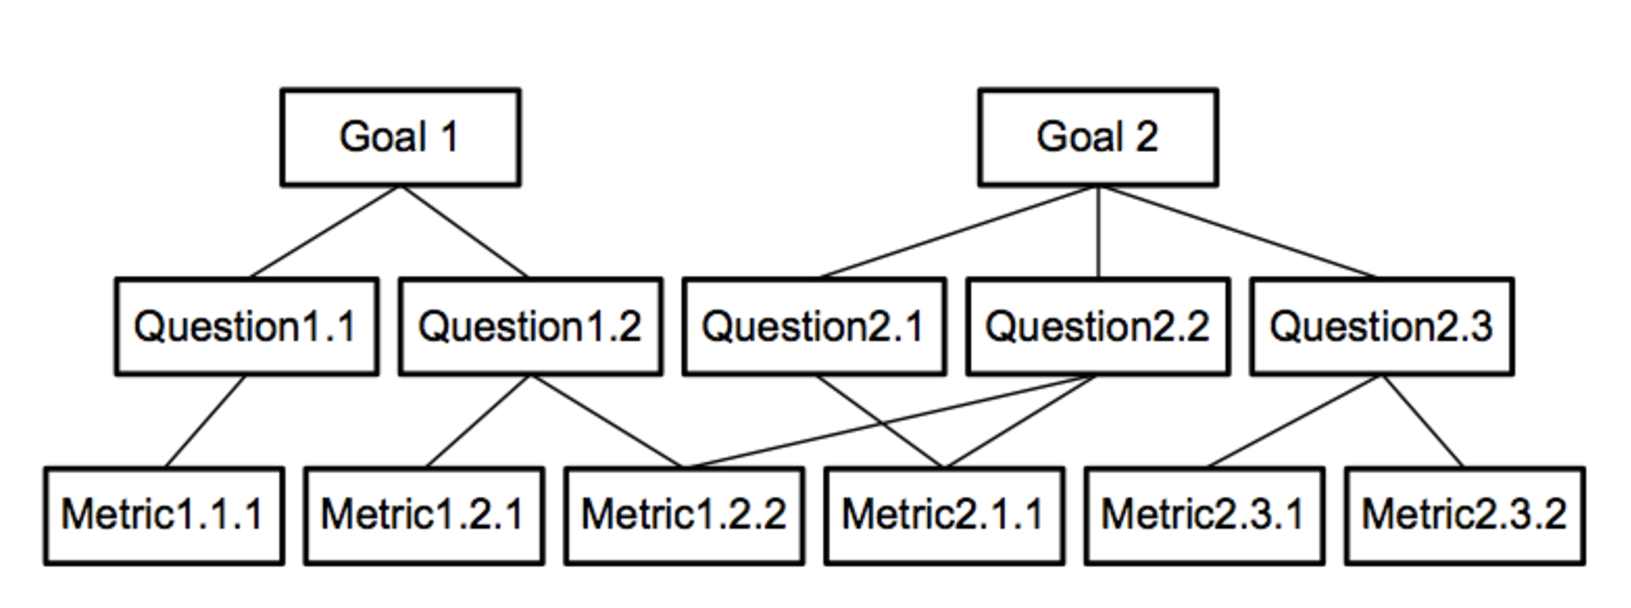
\includegraphics[width=10cm]{5-Evaluation/Figures/gqm.pdf}
    \end{center}
    \caption{\label{fig:gqm} ساختار روش هدف-پرسش-معیار }
\end{figure*}

\section{ارزیابی تغییرپذیری}
در این بخش به ارزیابی تغییرپذیری سیستم تحت طراحی بر اساس تبادل ناهمگام پیغام می‌پردازیم. برای ایجاد امکان ارزیابی کمّی تغییرپذیری، می‌توان از معیارهای کیفیت نرم‌افزار\LTRfootnote{Software Quality Metrics} استفاده کرد. این معیارها خصوصیاتی از قبیل پیچیدگی، قابلیت استفاده‌ی مجدد و آزمون‌پذیری یک سیستم را به صورت کمّی قابل سنجش و مقایسه می‌کنند. در ادامه با توجه به روش هدف-پرسش-معیار، عناصر ارزیابی تغییرپذیری سیستم را تعیین می‌کنیم.

\subsection{هدف}
در این ارزیابی هدف ارزیابی تغییرپذیری طراحی به روش تبادل ناهمگام پیغام است. این ارزیابی از طریق مقایسه‌ی نسخه‌های پیاده سازی شده‌ی سیستم آموزش ساده (بخش \ref\label{section:eduIntro}) به دو روش طراحی تبادل ناهمگام پیغام و طراحی متداول شیءگرا صورت می‌پذیرد.

\subsection{پرسش‌ها}
برای این ارزیابی ۳ پرسش در نظر گرفته می‌شود:
\begin{enumerate}
\item سیستم طراحی شده به روش تبادل ناهمگام، از نظر معیارهای کیفیت نرم‌افزار چگونه با سیستم طراحی شده به روش شیءگرا مقایسه می‌شود؟
\item اعمال تغییر قواعد منطق برنامه روی کدام نوع طراحی مشکل‌تر است؟ 
\item اعمال تغییر در مدل دامنه‌ی سیستم روی کدام نوع طراحی مشکل‌تر است؟ 
\end{enumerate}

\subsection{معیارها}
 به منظور پاسخ به هر کدام از پرسش‌های بالا می‌توان از معیارهای کیفیت در برنامه‌نویسی شیءگرا  استفاده کرد. پاسخ به پرسش اول مستقیماً با مقایسه‌ی معیارها پاسخ داده می‌شود. برای پرسش به پاسخ دوم، تغییرات منطق دامنه انتخاب و در هر دو سیستم اعمال می‌شوند و میزان تغییر هر کدام از معیارهای کیفیت بررسی و مقایسه می‌شود. برای پاسخ به پرسش سوم نیز به طریق مشابه می‌توان مقایسه را بعد از اعمال تغییر در مدل دامنه انجام داد. 
 معیارهای مختلفی برای بررسی کیفیت برنامه‌های شیءگرا در پژوهش‌های مختلف ارائه شده‌اند که از آن جمله می‌توان به معیارهای ابریو\LTRfootnote{Abreu}\cite{quality_metrics_1,quality_metrics_2}، معیارهای بانسیا و همکاران\LTRfootnote{Bansia et al}\cite{quality_metrics_3} و معیارهای چیدامبر و کمرر\LTRfootnote{Chidamber and Kemerer} که به متریک‌های سی‌کِی معروف هستند \cite{quality_metrcs_ck}. در این پژوهش تعدادی از متریک‌های موجود برای ارزیابی انتخاب شده‌اند. این انتخاب بر اساس میزان ارجاع در پژوهش‌های مختلف به این متریک‌ها و نیز تناسب آنها با طراحی‌های این پژوهش انجام شده است. مقاله‌ی \cite{metrics_stateOfTheArt} اطلاعات کاملی از متریک‌های مختلف کیفیت نرم‌افزار و میزان ارجاع به آنها را ارائه کرده است. معیارهای انتخاب شده برای بررسی تغییرپذیری برنامه در ادامه معرفی شده‌اند. در تعاریف و توضیحات این معیارها از مقاله‌ی \cite{metrics_stateOfTheArt} بهره گرفته شده است.
\begin{enumerate}
\item\textbf{تعداد کلاس:}
 تعداد کلاس‌های پیاده‌سازی شده (بدون در نظر گرفتن کلاس‌های داخلی)
\item\textbf{میانگین تعداد متد در هر کلاس}

\item\textbf{میانگین تعداد فیلد تعریف شده در هر کلاس}

\item\textbf{تعداد خطوط متن برنامه}

\item\textbf{میانگین تعداد خطوط متن هر کلاس}

\item\textbf{میانگین پیچیدگی چرخه‌ای \lr{(CC)}\LTRfootnote{Average Cyclomatic Complexity}:}
پیچیدگی چرخه‌ای یک متد برابر است با تعداد نقاط تصمیم در گراف کنترل آن بعلاوه‌ی یک. نقاط تصمیم در یک متد در شرط‌ها و حلقه‌ها و دستورهای مشابه رخ می‌دهند. به عنوان مثال، پیچیدگی چرخه‌ای برای یک متد که یک بلوک شرط \lr{(if)} یا یک حلقه دارد عدد ۲ است و برای متدی که صرفاً دستورات خطی دارد عدد ۱ است. هرچه عدد پیچیدگی چرخه‌ای بزرگتر باشد برنامه به موارد آزمون بیشتری نیاز دارد.
\item\textbf{میانگین متدهای وزن‌دار در کلاس\LTRfootnote{Average Weighted Methds per Class}:}
تعداد متدهای وزن‌دار در یک کلاس برابر است با جمع پیچیدگی چرخه‌ای متدهای آن کلاس.
\item\textbf{میانگین عمق درخت وراثت \lr{(DIT)}\LTRfootnote{Average Depth of Inheritance Tree}:}
عمق درخت وراثت برابر است با تعداد کلاس‌هایی که در زنجیره‌ی وراثت یک کلاس آن را به ریشه می‌رساند.

\item\textbf{میانگین تعداد فرزندان:}
تعداد فرزندان یک کلاس برابر است با تعداد کلاس‌هایی که در زنجیره‌ی وراثت کلاس پایین‌تر از خود کلاس هستند.
\item\textbf{میانگین \gls{جفت‌شدگی}\LTRfootnote{Coupling} بین اشیاء:}
یک کلاس با کلاس دیگر جفت‌شدگی دارد اگر یکی از دو کلاس (یا هردو) متدی از دیگری را فراخوانی کرده باشد. معیار جفت‌شدگی بین اشیاء برای یک کلاس برابر است با تعداد کلاس‌های که با کلاس مورد نظر جفت‌شدگی دارد. (معیار انتخاب شده میانگین این عدد در بین همه‌ی کلاس‌ها است.)
\end{enumerate}

\subsection{نتایج ارزیابی}
\subsubsection{پرسش اول}
برای پاسخ به پرسش اول، معیارهای انتخاب شده در پیاده‌سازی‌های سیستم آموزش ساده (بخش \ref\label{section:eduIntro}) به دو روش تبادل ناهمگام پیغام و شیءگرا محاسبه شده و باهم مقایسه شده‌اند. نتیجه‌ی این مقایسه در جدول \ref{table:mod_result_1} ارائه شده است.


%%%%%%%%%%%%%%%%%%%%%%%%%%%%%
%%%%  Q1 results
%%%%%%%%%%%%%%%%%%%%%%%%%%%%%
\begin{table}
\begin{center}
\begin{tabular}{|p{7cm}|p{4cm}|p{4cm}|}
	\hline
%	\multicolumn{1}{|p{7cm}}{Header 1} & \multicolumn{1}{p{4cm}}{Header 2} & \multicolumn{1}{p{4cm}|}{Header 3} \\
%\multicolumn{1}{|p{7cm}}{\textbf{معیار}} & \multicolumn{1}{|p{4cm}}{\textbf{مقدار معیار برای طراحی به روش شیءگرا}} & \multicolumn{1}{|p{4cm}|}{\textbf{مقدار معیار برای طراحی به روش تبادل ناهمگام پیغام}} \\
\textbf{معیار} & \textbf{مقدار معیار برای طراحی به روش شیءگرا} & \textbf{مقدار معیار برای طراحی به روش تبادل ناهمگام پیغام} 
\\ 
	\hline
	تعداد کلاس
	 &
\centering	 ۱۵
	 &
\centering	 ۱۷
\\
	\hline
	میانگین تعداد متد در هر کلاس
	 &
\centering	 ۶/۲
	 &
\centering	 ۵/۱۱
\\
	\hline
	میانگین تعداد فیلد تعریف شده در هر کلاس
	 &
\centering	 ۱.۹۳
	 &
\centering	 ۴.۲۹
\\
	\hline

	تعداد خطوط متن برنامه
	 &
\centering	 ۶۶۴
	 &
\centering	 ۷۶۰
\\
	\hline
	
		میانگین تعداد خطوط متن هر کلاس
	 &
\centering	 ۴۴.۲۷
	 &
\centering	 ۴۲.۲۲
\\
	\hline
	
		میانگین پیچیدگی چرخه‌ای
	 &
\centering	 ۱.۵۸
	 &
\centering	 ۱.۲۵
\\
	\hline
	
		میانگین متدهای وزن‌دار در کلاس
	 &
\centering	 ۹.۸
	 &
\centering	 ۷.۱۲
\\
	\hline
	
		میانگین عمق درخت وراثت
	 &
\centering	 ۱.۳۳
	 &
\centering	 ۱.۵۹
\\
	\hline
	
		میانگین تعداد فرزندان
	 &
\centering	 ۰.۳۳
	 &
\centering	 ۰.۵۹
\\
	\hline
	
			میانگین جفت شدگی بین اشیاء
	 &
\centering	 ۳.۶
	 &
\centering	 ۳.۱۸
\\
	\hline
\end{tabular}
\caption{\label{table:mod_result_1} مقادیر معیارها برای پرسش اول}
\end{center}
\end{table}










\section{ارزیابی کارایی}
سبیس
سبیس
\subsection{بررسی معیارهای  ایستا }
با توجه به بزرگی سیستم مورد مطالعه، برای این مطالعه‌ی موردی دو مورد کاربرد از مجموعه‌ی مهم‌تری
\subsection{اعمال تغییرات}
\subsubsection{تغییر اول}

\section{نتایج ارزیابی}
قبل از بررسی نتایج، لازم است برخی نکات در مورد اجرای آزمون‌ها مورد بررسی قرار گیرد. مطابق آن‌چه در فص

\subsection{تحلیل نتایج}
با داشتن نتای